\chapter{Análisis y Diseño}
En este capítulo se presenta el problema de diseño de rutas con POIs y modelización. Para resolver el problema, se proponen inicialmente dos métodos heurísticos que permitirán evaluar el funcionamiento del prototipo. Además se detallarán los aspectos más importantes relacionados con el diseño del prototipo.
\section[Análisis]{Análisis}
\subsection[Diseño de rutas turísticas]{Diseño de rutas turísticas}
Los problemas de diseño de rutas turísticas (Tourist Trip Design Problems, TTDP) consisten en seleccionar los POIs (points of interest / puntos de interés ) a visitar por un turista atendiendo a sus restricciones y al beneficio o grado de satisfacción que produce su visita. El turista dispone en su estancia de un cierto número de días para organizar las visitas a los POIs mediante rutas de duración limitada. Se parte de un conjunto de puntos disponibles a visitar de los que se conoce, el beneficio o grado de satisfacción, la duración de la visita y el intervalo de tiempo en el que puede realizarse. El beneficio total que intenta maximizar el turista es la suma de los beneficios obtenidos en cada visita.\newline
Los elementos que forman parte del modelo son:
\begin{itemize}
	\item Un conjunto de POIs , asociado a un índice $i, i=1,2,...,n$ y con los siguientes atributos:
	\begin{itemize}
		\item Una puntuación o beneficio $s_i$.
		\item Un tiempo de duración de la visita $r_i$.
		\item Un intervalo de tiempo $[e_i,l_i]$ dentro del que se puede realizar la visita.
	\end{itemize}
	\item Un punto de partida de cada una de las rutas denotado por $i=0$.
	\item Los tiempos de recorrido entre los pares de puntos $t_{ij}, i,j=0,1,...,n$.
	\item Un tiempo máximo $T_{max}$ de duración total de la ruta del día considerando los tiempos de viaje, visita y espera en los POI.
	\item Una función objetivo $max \sum_{i=1}^{n}s_iy_i^k$ \newline
	En la que $y_i$ corresponde a una variable de visita para cada uno de los POIs $i, i=1,...,n$. Dicha variable es binaria, teniendo como valor 1 si el punto de interés $i$ es visitado en la ruta y un 0 si no se visita. Esta variable solamente tendrá valor 1 si además está disponible cuando se quiere visitar dicho punto de interés, es decir, si el punto se va a visitar durante el intervalo de tiempo $[e_i,l_i]$ asociado a la variable.
\end{itemize}
El problema de optimización coincide con el Team Orienteering Problem with Time Windows (TOPTW) que se ha estudiado en la literatura científica con algunas modificaciones. Se consideran POIs museos, miradores, catedrales, mezquitas, etc... de la ciudad que el usuario elija antes de iniciar el algoritmo; además, dicho POIs son considerados para la ruta de un único día.
\subsection[Heurísticas propuestas]{Heurísticas propuestas}
Como solución inicial a este problema se ha utilizado una heurística Greedy, ya que es una heurística rápida que puede ejecutar cualquier dispositivo móvil. Dicha huerística Greedy seleccionará siempre el punto más cercano al punto de interés actual; este proceso se repetirá hasta que no puedan introducirse más POIs en la solución, bien porque no haya más POIs por visitar o bien porque no haya más tiempo para visitarlos. El pseudocódigo de dicho algoritmo es el siguiente:\newline
\begin{algorithm}[H]
	\caption{Pseudocódigo algoritmo Greedy.}
	\label{alg:greedy_alg}
	\begin{algorithmic}
		\Function{Greedy}{lista\_POI}
		\While( es posible visitar POI)
		\State mejor\_poi $\gets$ encontrarMásCercano(último\_poi\_visitado, tiempo\_actual) 
		\State tiempo\_entrada$\gets$tiempo\_actual$+$tiempo\_llegada(último\_poi\_visitado,mejor\_poi)
		\State tiempo\_salida $\gets$ tiempo\_entrada $+$ tiempo\_visita\_mejor\_poi
		\State solución.añadir(mejor\_poi,tiempo\_entrada, tiempo\_salida)
		\State tiempo\_actual $\gets$ tiempo\_salida
		\State eliminar mejor\_poi de la lista de POI disponibles
		\EndWhile
		\State \textbf{return} solución
		\EndFunction
	\end{algorithmic}
\end{algorithm}
\vspace{0.06in}
El parámetro \enquote*{lista\_POI} es la lista de POIs seleccionados para realizar la búsqueda, los cuales se van a usar para buscar la ruta en el algoritmo.\newline

La función \textit{encontrarMásCercano(último\_poi\_visitado, tiempo\_actual)} encuentra el punto de interés más cercano al último punto de interés seleccionado y que se pueda visitar en el momento que se sale del último punto de interés, es decir, que el tiempo de entrada a dicho punto de interés esté dentro del intervalo de tiempo permitido para dicho punto de interés. Para ello, recorre un vector que contiene el tiempo necesario para llegar desde el último punto de interés visitado y otro punto; de todos los POIs que estén disponibles, selecciona aquel cuyo tiempo de llegada desde el último punto de interés sea menor. Dicho vector está contenido en una matriz que guarda esta información por cada uno de los POIs. Un punto de interés está disponible si está abierto a la hora en la que el algoritmo lo vaya a seleccionar y si no está incluido en la solución.\newline

Dentro del pseudocódigo se pueden ver tres variables que tienen que ver con el tiempo; la variable \enquote*{tiempo\_actual} guarda el tiempo actual en cada momento del algoritmo, es decir, es una variable que va actualizando su valor cada vez que se selecciona un nuevo punto de interés. La variable \enquote*{tiempo\_entrada} representa el tiempo de entrada aproximado al punto de interés seleccionado; este valor se calcula con el valor de \enquote*{tiempo\_actual} más el tiempo necesario para llegar desde dicho punto hasta el punto seleccionado, representado por la función \enquote*{tiempo\_llegada(último\_poi\_visitado,mejor\_poi)}. Por último, la variable \enquote*{tiempo\_salida} representa el tiempo aproximado de salida de dicho punto de interés, esta variable se calcula como la suma de \enquote*{tiempo\_entrada} y el tiempo aproximado de visita, representado por la variable  \enquote*{tiempo\_visita\_mejor\_poi}.\newline

Una vez termina el algoritmo, devuelve la solución. Dicha solución cuenta con un vector que contiene los identificadores de los POIs seleccionados; además, contiene la hora aproximada de entrada y salida de cada uno de los POIs seleccionados. Además, los POIs contenidos en la solución, se encuentran ordenados por orden en llegada.\newline

Como otra posible heurística que resuelva el problema y que no necesite de mucho tiempo de cómputo, se ha propuesto también la metaheurística constructiva GRASP (Greedy Randomized Adaptive Search Procedure). Dicha metaheurística comprende dos fases: una fase constructiva y otra de búsqueda local. En la fase constructiva se genera una solución partiendo de una ruta vacía a la que se va añadiendo POIs desde una Lista Restringida de Candidatos (Restricted Candidate List, RCL en inglés) de forma aleatoria hasta que no se puedan añadir nuevos puntos a la ruta. En la fase de búsqueda local se reemplaza la solución obtenida en la parte constructiva por la mejor de sus soluciones vecinas si existe mejora. Estas dos fases se ejecutan un cierto número de iteraciones.\newline

Ahora se mostrará el pseudocódigo del algoritmo, y de cada una de las fases en inglés.
\vspace{0.06in}

\begin{algorithm}
	\caption{Pseudocódigo algoritmo GRASP.}
	\label{alg:grasp}
\begin{algorithmic}
	\Function{GRASP}{maxIteraciones,tamRCL}
	\State $ leerDatos() $
	\For{$i=1$ to maxIteraciones}
		\State solución $ \gets $ GRASPFaseConstructiva(tamRCL)
		\State  solución $\gets$ BúsquedaLocal(solución)
		\If{solución $\geq$ mejorSolución}
			\State  mejorSolución $\gets$ solución
		\EndIf
	\EndFor
	
	\State \textbf{return} mejorSolución
	\EndFunction
\end{algorithmic}
\end{algorithm}

\vspace{0.06in}
Para la parte constructiva del algoritmo, primero crearemos una lista de candidatos (CL), la cual tiene un tamaño igual al de la lista de POIs que queden disponibles. Dicha lista de candidatos contiene la posición dentro de la lista de POIs y la puntuación que tiene dicho punto de interés según las preferencias elegidas por el usuario. La forma de puntuar un punto de interés dependerá también del tiempo necesario para llegar desde el último punto de interés seleccionado y dicho punto de interés. Al igual que para la heurística Greedy, solo se considerarán aquellos POIs que estén disponibles, es decir, que no estén incluidos ya en la solución que se está construyendo y que estén abiertos en el momento que pueden ser seleccionados.\newline

Una vez hemos calculado la lista de candidatos, se crea la lista restringida de candidatos con los POIs mejor valorados, esta es de tamaño \enquote*{tamRCL}. Una vez hemos obtenido la lista de candidatos restringida, elegimos uno de los POIs de forma aleatoria y lo introducimos dentro de la solución. Este proceso se repite hasta que no se puedan introducir más POIs dentro de la solución. El pseudocódigo de este algoritmo es el siguiente.\newline

\vspace{0.06in}
\begin{algorithm}
	\caption{Pseudocódigo algoritmo GRASPFaseConstructiva.}
	\label{alg:grasp_contruct}
	\begin{algorithmic}
		\Function{GRASPFaseConstructiva}{tamRCL}
		\State solución.añadir(nodo\_salida)
		\While{es posible visitar POIs}
			\For{cada poi en lista\_POIs}
				\State valor $\gets$ f(poi)
				\State CL.añadir([valor,i])
			\EndFor
			\State Crear RCL con los mejores tamRCL elementos de CL
			\State seleccionado $\gets$ seleccionarRandom(RCL)
			\State solución.añadir(lista\_POIs[seleccionado.i])
		\EndWhile
		\State \textbf{return} solución
		\EndFunction
	\end{algorithmic}
\end{algorithm}
\vspace{0.06in}

En este algoritmo, la función llamada \enquote*{f(poi)} devuelve el valor de dicho POI, dicho valor esta representado por el tiempo necesario para llegar desde el último punto visitado hasta dicho punto \enquote*{poi}. La variable \enquote*{i} representa la posición del POI dentro de \enquote*{lista\_POIs}, utilizada para acceder directamente a la información de dicho POI dentro de \enquote*{lista\_POIs}. La variable \enquote*{seleccionado} representa el elemento seleccionado de la lista \enquote*{RCL} (un par que contiene el valor de dicho POI y la posición dentro de \enquote*{lista\_POIs}) de forma aleatoria.\newline

Para la fase de optimización se utilizará el algoritmo de búsqueda local, dicho algoritmo busca la mejor solución posible entre la solución actual y los vecinos de esta. Una solución vecina es aquella que intercambie dos POIs dentro de la solución, por ejemplo, el segundo por el cuarto. El procedimiento es el siguiente, se generan todos los posibles vecinos de la solución, y por cada uno de ellos se comprueba si la valoración de dicha solución vecina es mejor que la mejor solución actual; finalmente se devuelve la mejor solución encontrada. El pseudocódigo del algoritmo es el siguiente.\newline

\begin{algorithm}[H]
	\caption{Pseudocódigo algoritmo BúsquedaLocal.}
	\label{alg:local_search}
	\begin{algorithmic}
		\Function{BúsquedaLocal}{solución}
		\ForAll{solución\_vecina de solución}
		\If{solución\_vecina $\geq$ solución}
			\State solución $\gets$ solución\_vecina
		\EndIf
		\EndFor
		\State \textbf{return} solución
		\EndFunction
	\end{algorithmic}
\end{algorithm}

\vspace{0.06in}
Para generar un nuevo vecino de la solución dada, se intercambiarán la posición de dos POIs dentro de la solución. Además de intercambiar dichos puntos, hay que actualizar los valores de entrada y de salida de dichos puntos y comprobar que la solución sigue siendo válida. Es decir, que sigue respetando el número de POIs que hay en la solución y que la hora en la que se finaliza la ruta sigue siendo la misma.

\chapter{Diseño}
En este capítulo se detalla la arquitectura del sistema.
\section[Diagrama de clases]{Diagrama de clases}
En este apartado se mostrarán los diagramas de clases de los elementos más importantes de la aplicación.\newline

La primera figura que se muestra es el diagrama de clases del Fragment \enquote{TypesFragment} \ref{fig:fragment_diagram}. Dicho diagrama de clases muestra las siguientes clases:
\begin{itemize}
	\item La clase \textbf{TypesFragment}:esta clase es la encargada de comunicar los elementos gráficos que se encuentra dentro de la lista de alojamientos y puntos de interés, también del botón que inicia el algoritmo de búsqueda de la ruta óptima.
	\item La clase \textbf{TypesRecyclerFragment}: es la encargada de manejar la lista de alojamientos y puntos de interés, además devuelve los elementos seleccionados en la lista al iniciar la búsqueda de la ruta. También se encarga de gestionar la interfaz gráfica de la lista.
	\item La clase \textbf{CityNodesViewHolder}: es la encargada de gestionar los elementos gráficos de los puntos de interés o los alojamientos de forma individual.
	\item La clase \textbf{TypeViewHolder}: es la encargada de gestionar los elementos gráficos de los tipos que aparecen en la lista de alojamientos y puntos de interés.
	\item La clase \textbf{CityNode}: clase que contiene toda la información importante sobre un alojamiento o punto de interés que se muestra en la lista.
	\item La clase \textbf{TypeOfNode}: clase que contiene la información sobre un tipo de nodo de interés.
\end{itemize}
\vspace{0.06in}
En la segunda figura  \ref{fig:main_activity_diagram}, se muestra el diagrama de clases de la actividad principal de la aplicación. Las clases que se muestran en el diagrama son las siguientes:
\begin{itemize}
	\item La clase \textbf{MapsActivity} es la clase clase principal y gestiona el mapa que se muestra y se comunica con la clase \textbf{TypesFragment} para obtener los nodos seleccionados. Esta clase contiene vectores que almacenan información sobre los marcadores que aparecen en el mapa. Dicha información se utiliza también para obtener la matriz de distancias. También contiene otros vectores para almacenar la información contenida en la solución, dichos vectores se utilizan para mandar la información de la solución a la actividad ResultActivity.
	\item La clase \textbf{DownloadFileFromURL}: se encarga de descargar y guardar la información que devuelven las peticiones a los servidores sobre alojamientos, puntos de interés, rutas y matriz de tiempos entre puntos de interés. Esta clase hereda de la clase AsyncTask, lo cual le permite ejecutarse en segundo plano sin que afecte al rendimiento de la interfaz de usuario.
	\item La clase \textbf{jsonProcessor} se encarga de procesar la información que se ha guardado en ficheros tras ser descargada. Esta clase utiliza la clase \textbf{JsonParser} para procesar los archivos. Además, también hereda de la clase AsyncTask por lo que se ejecuta en segundo plano.
	\item La clase \textbf{JsonParser} se encarga de procesar archivos JSON y devuelve la información contenida en los archivos en estructuras que la aplicación puede manipular.
	\item La clase \textbf{SendNodes} se encarga de obtener la matrix de distancias entre los puntos de interés selecionados. Para ello utiliza las clases \textbf{DownloadFileFromURL} y\textbf{ jsonProcessor}, también se ejecuta en segundo plano debido a que hereda de la clase AsyncTask.
	\item La clase\textbf{ FindSolution} se encarga de ejecutar en segundo plano el algoritmo de búsqueda de rutas y de mandar la solución a la siguiente actividad. Para ello hace uso de la clase \textbf{PathFinder} y la clase \textbf{Solution}.
	\item La clase \textbf{PathFinder} es la clase que contiene el algoritmo de búsqueda de rutas. Dicha clase obtiene la solución al problema mediante un algoritmo Greedy y devuelve un objeto de la clase \textbf{Solution}.
	\item La clase \textbf{Solution} es la que clase que contiene una solución al problema. Esta clase cuenta con un vector que almacena los identificadores de los puntos de la solución, así como dos vectores que almacenan las horas de entrada y de salida de cada uno de los puntos de la solución.
\end{itemize}
\vspace{0.06in}
En la tercera figura \ref{fig:models_diagram}, se muestra el diagrama de clases del paquete models; dicho paquete está formador por clases que se utilizan para modelar diferentes estructuras dentro del proyecto. Las clases que aparecen en el diagrama son las siguientes:
\begin{itemize}
	\item La clase \textbf{Solution}: clase que contiene una solución al problema. Contiene vectores para almacenar identificadores y horarios de entrada y salida de los lugares por los que pasa la solución.
	\item La clase \textbf{ModelNode}: clase genérica que se utiliza para poder mostrar elementos tanto de la clase \textbf{CityNode} y \textbf{TypeOfNode}; ambas clases están explicadas en la descripción del primer diagrama de clases.
	\item La clase \textbf{SolutionNode}: clase que contiene el nombre, el horario de entrada y salida de un nodo de la solución. Esta clase se utiliza para encapsular los nodos de la solución y acceder a los datos a la hora de mostrar la lista de la solución.
\end{itemize}
\vspace{0.06in}
La cuarta figura \ref{fig:result_activity_diagram} muestra el diagrama de clases de la Activity ResultActivity, dicha Activity se muestra cuando se obtiene una solución. Las clases que se muestran en el diagrama son las siguientes:
\begin{itemize}
	\item La clase \textbf{ResultActivity}. Esta clase se ocupa de leer los datos mandados por la actividad principal y procesarlos para comunicarselos a la clase \textbf{SolutionFragment}.
	\item La clase \textbf{SimpleFragmentPagerAdapter}. Esta clase se ocupa de ver el número de soluciones que se han encontrado y crear un objeto de la clase \textbf{SolutionFragment} para mostrar cada una de ellas.
	\item La clase SolutionFragment. Esta clase se ocupa de mostrar en un mapa los marcadores de la solución y la lista con la información específica de cada uno de los marcadores. Además se ocupa de calcular el camino entre los distintos marcadores de la solución.
\end{itemize}
\vspace{0.06in}
Por último, en la quinta figura \ref{fig:solution_recycler_diagram} se muestra el diagrama de clases de la clase \textbf{SolutionFragment}. A continuación se describen cada una de las clases que se muestran en el diagrama:
\begin{itemize}
	\item La clase \textbf{SolutionFragment} se ha definido en la figura \ref{fig:result_activity_diagram} anterior. Es la encargada de gestionar todas las vistas que muestran la solución.
	\item La clase \textbf{FindRoutes}. Esta clase se encarga de mandar una petición a un servidor para obtener la ruta óptima entre los nodos de la solución y procesarla, después manda la información procesada a la clase \textbf{SolutionFragment} para que dibuje la ruta.
	\item La clase \textbf{SolutionRecyclerAdater} se encarga de manejar la lista con los nodos de la solución y de mostrarlos en una lista.
	\item La clase \textbf{SolutionNode}. Es una clase que contiene la información sobre un nodo de la solución.
	\item La clase \textbf{SolutionNodeViewHolder}. Es una clase que utiliza la información de un objeto de la clase \textbf{SolutionNode}  y la muestra dentro de la lista que gestiona la clase \textbf{SolutionRecyclerAdapter}.
\end{itemize}
\begin{figure}[H]
	\centering
	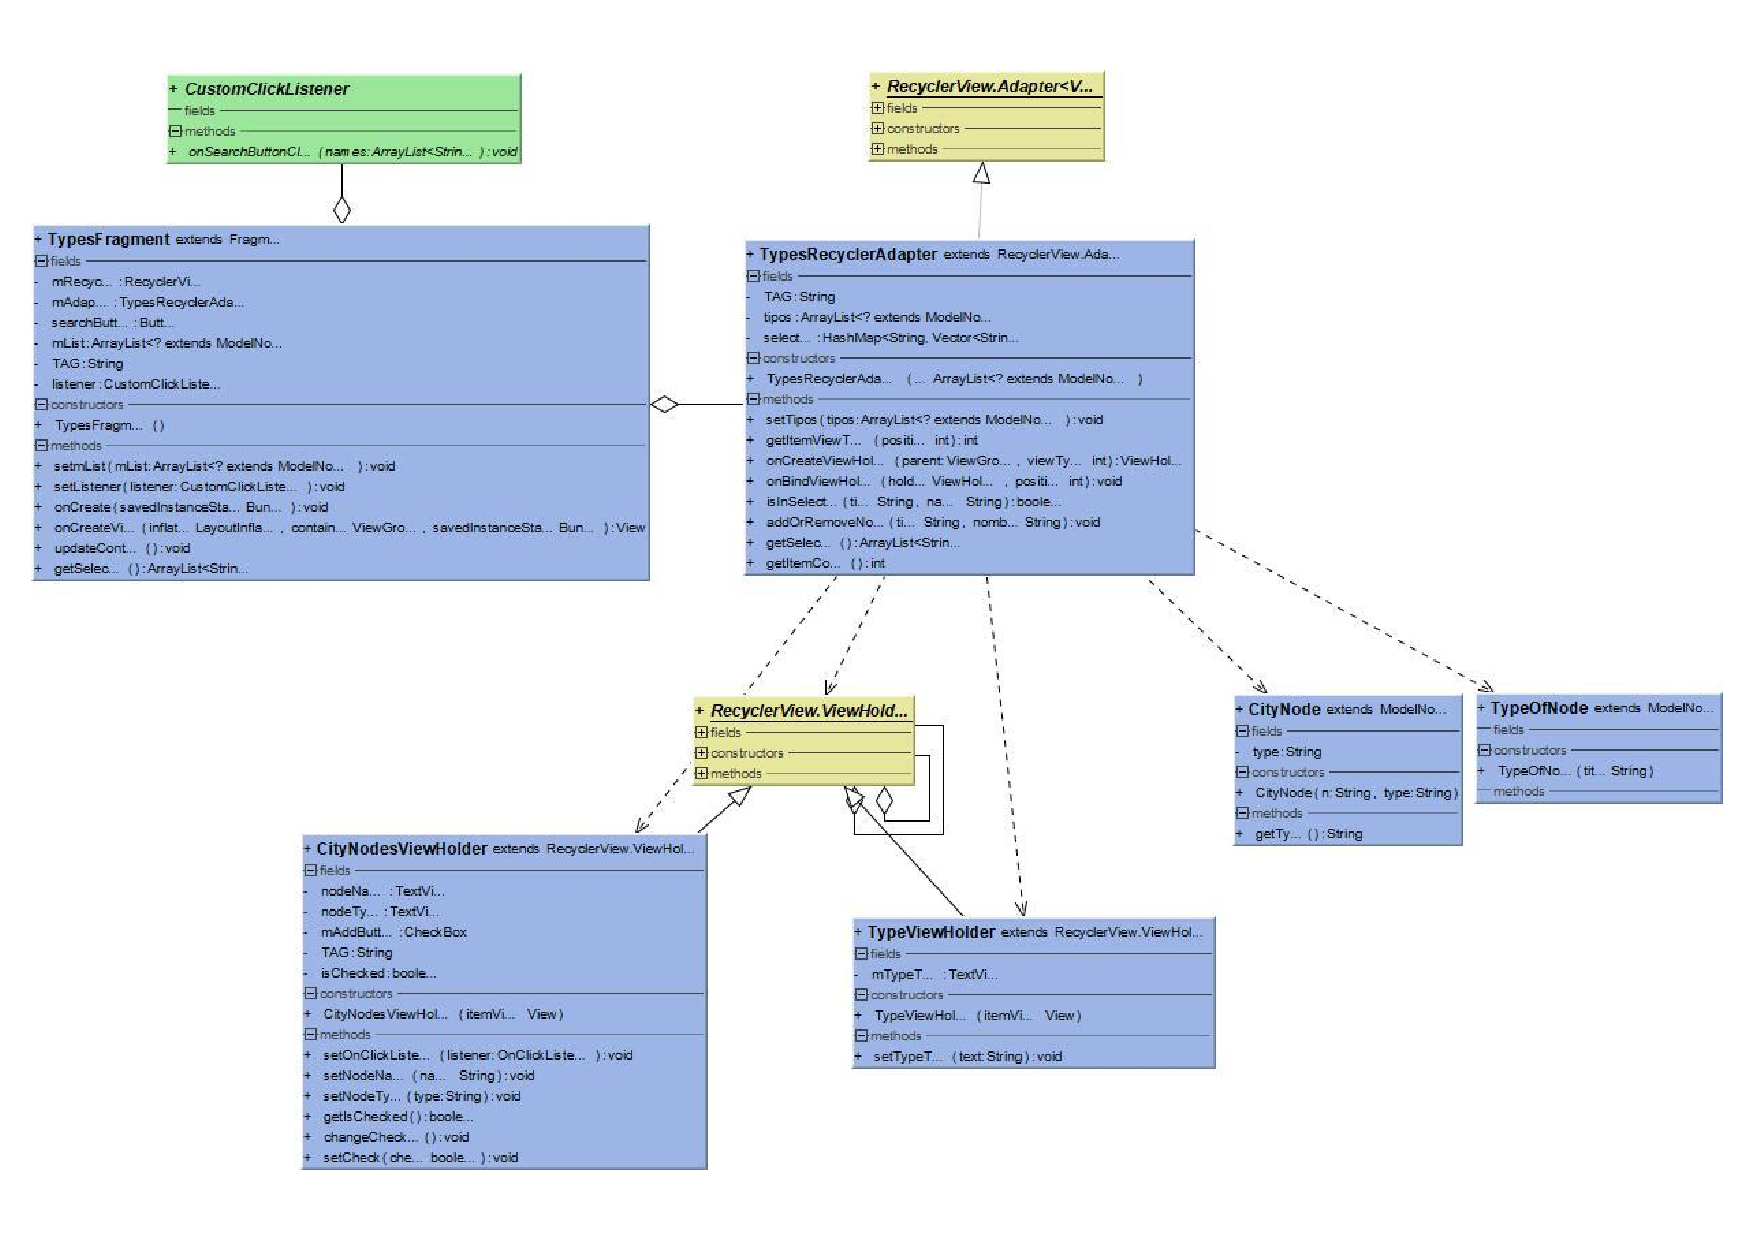
\includegraphics[scale=.8,angle=90]{imagenes/fragment_class_diagram.pdf}
	\caption{Diagrama de clases del \textbf{TypesFrament} }
	\label{fig:fragment_diagram}
\end{figure}
\begin{figure}[H]
	\centering
	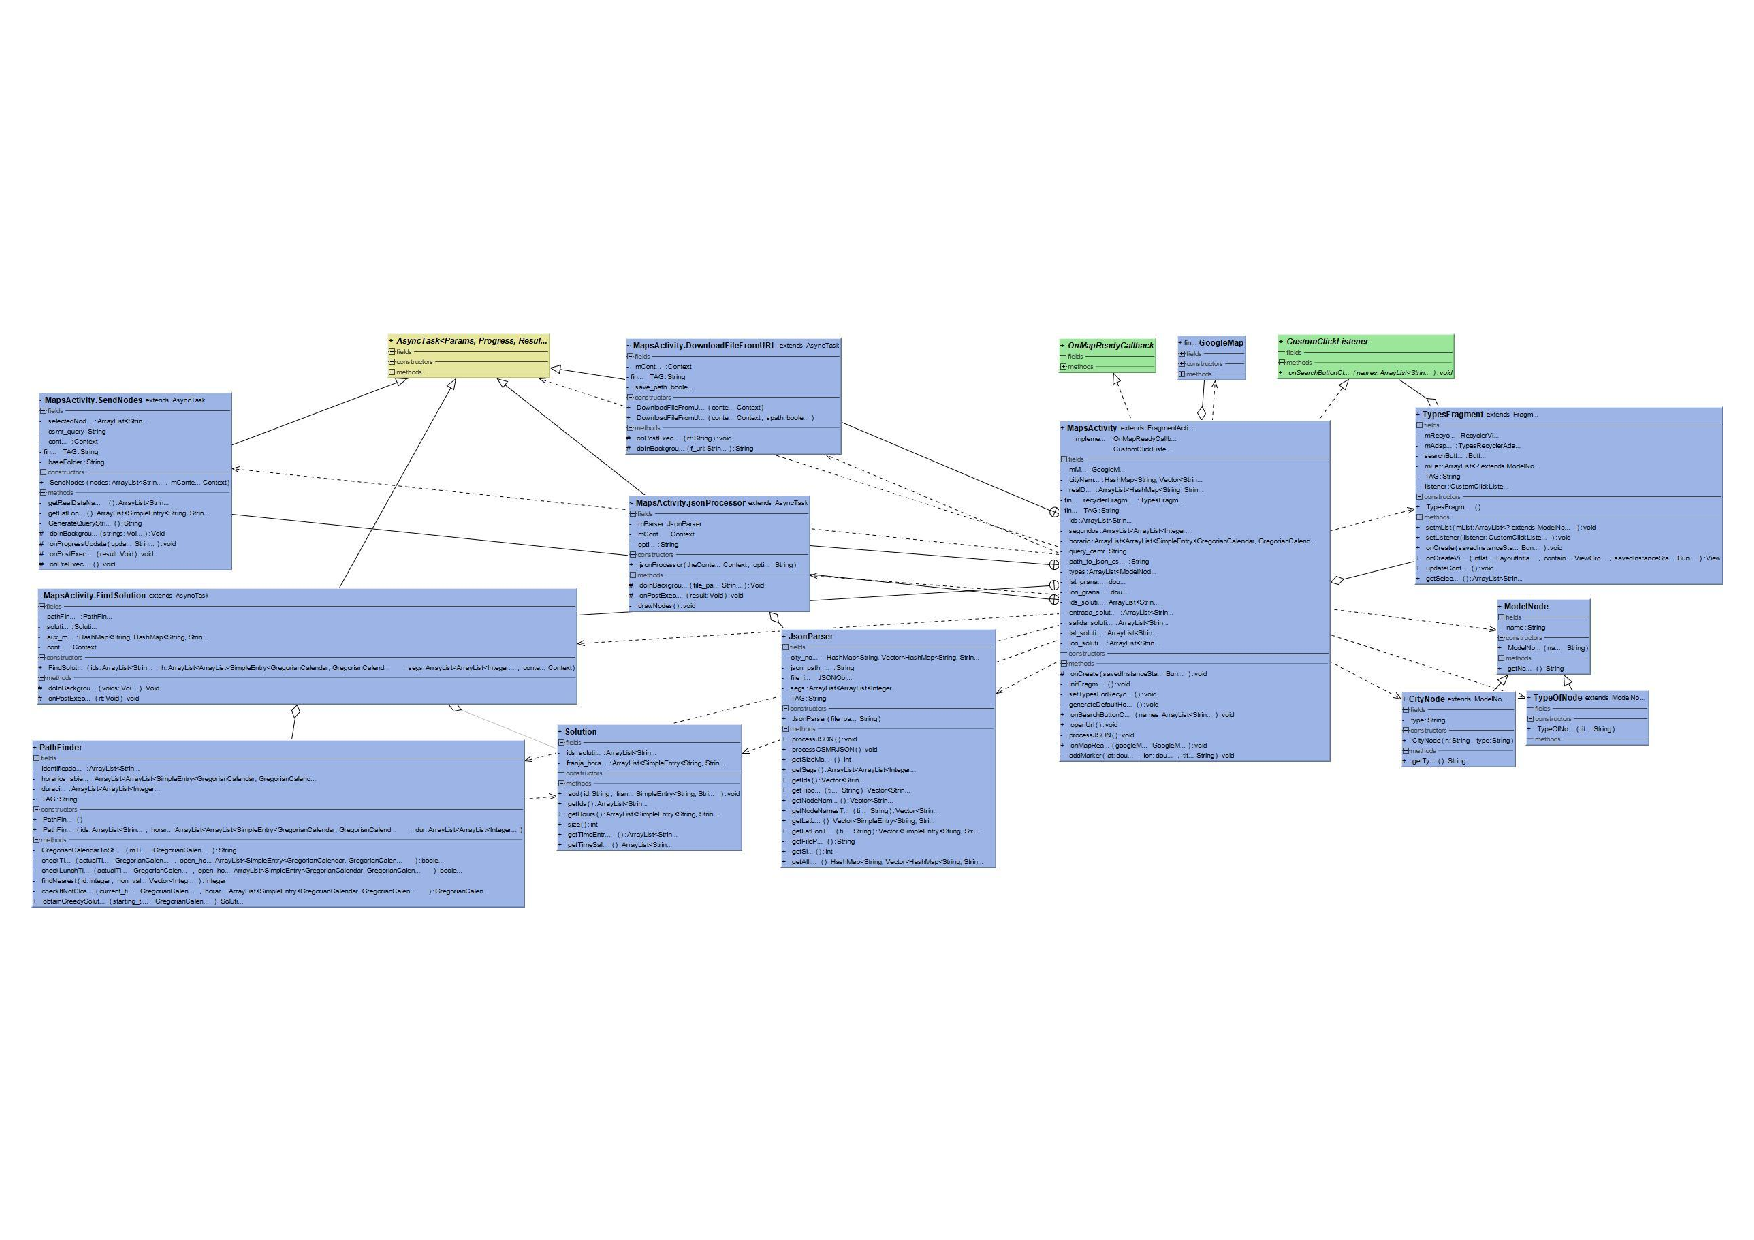
\includegraphics[scale=.8,angle=90]{imagenes/main_activity_class_diagram.pdf}
	\caption{Diagrama de clases de la actividad principal \ref{fig:anexo_diagrama_main_activity} }
	\label{fig:main_activity_diagram}
\end{figure}
\begin{figure}[H]
	\centering
	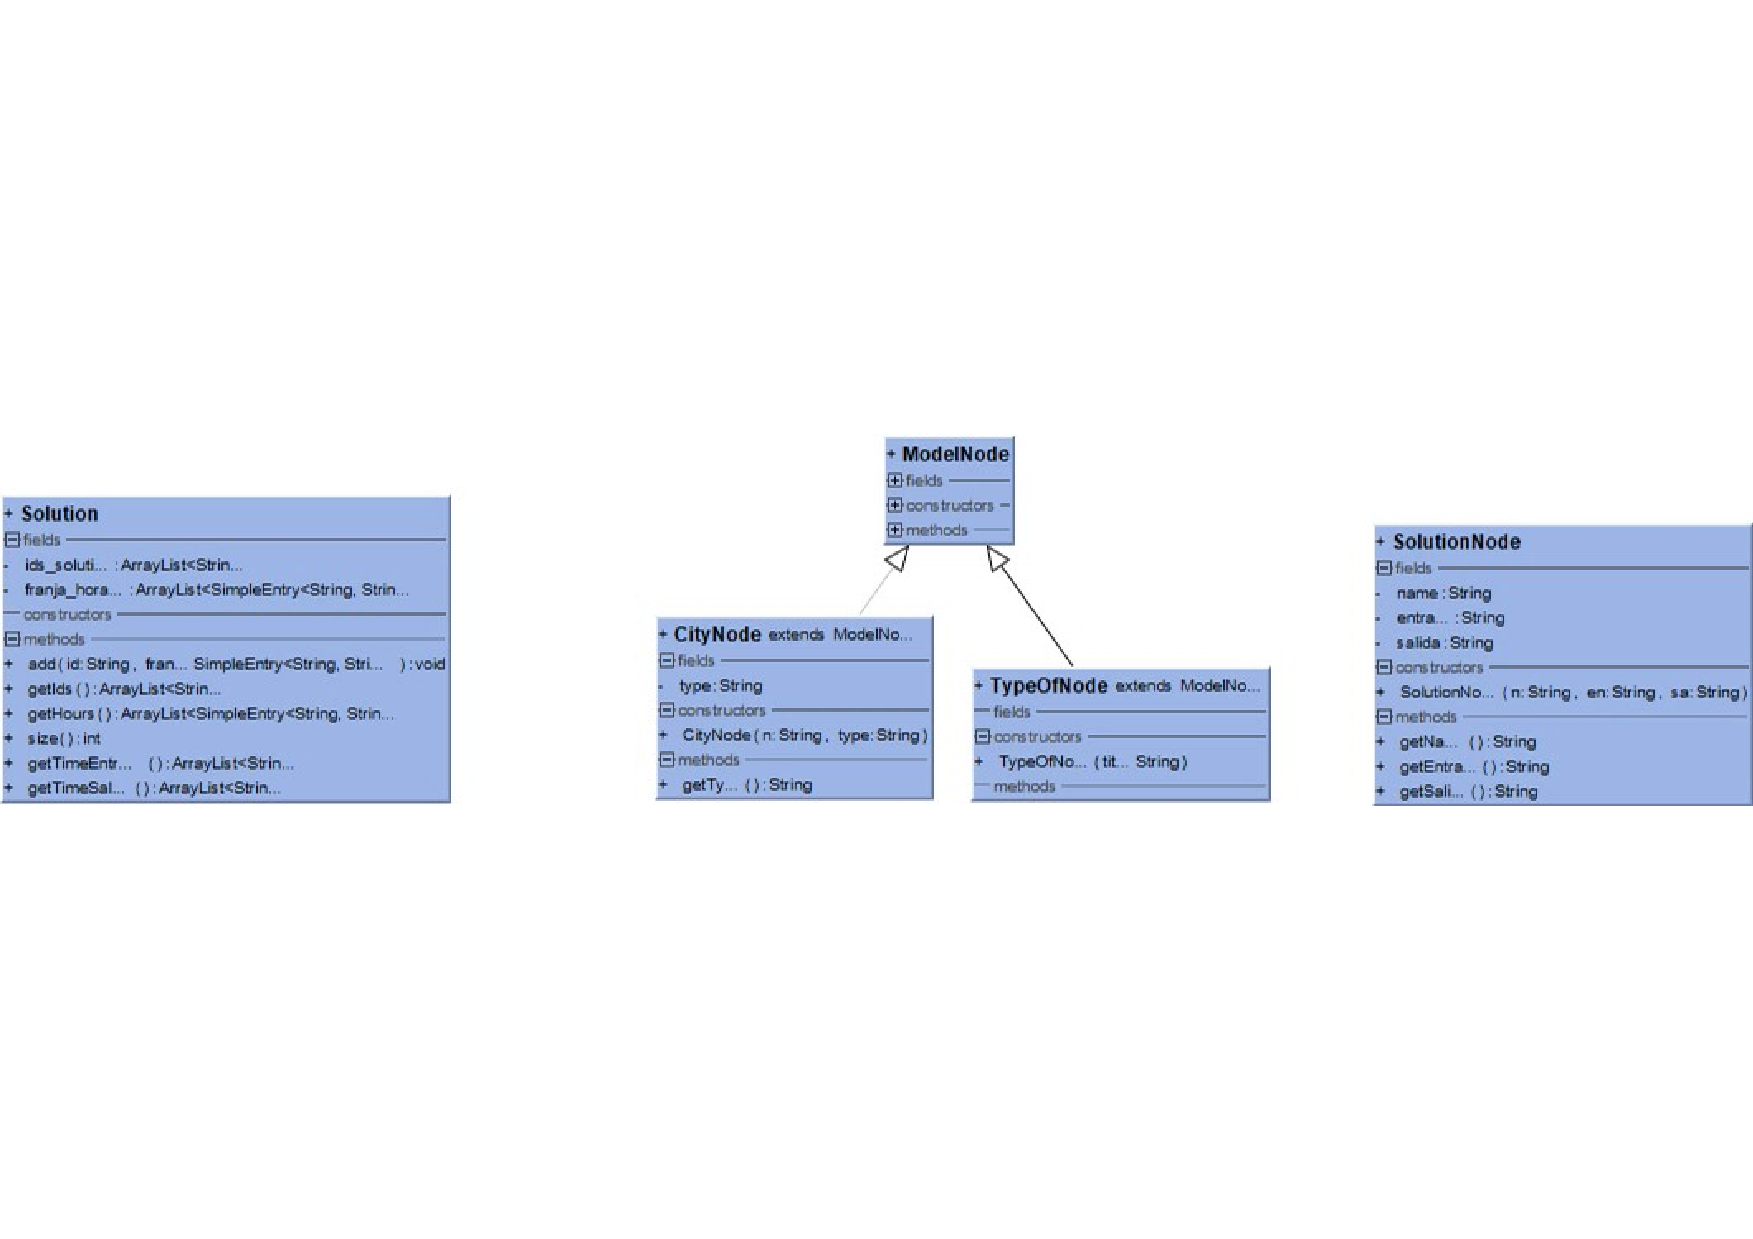
\includegraphics[scale=0.8,angle=90]{imagenes/models_package.pdf}
	\caption{Diagrama de clases del paquete \textbf{models}}
	\label{fig:models_diagram}
\end{figure}

\begin{figure}[H]
	\centering
	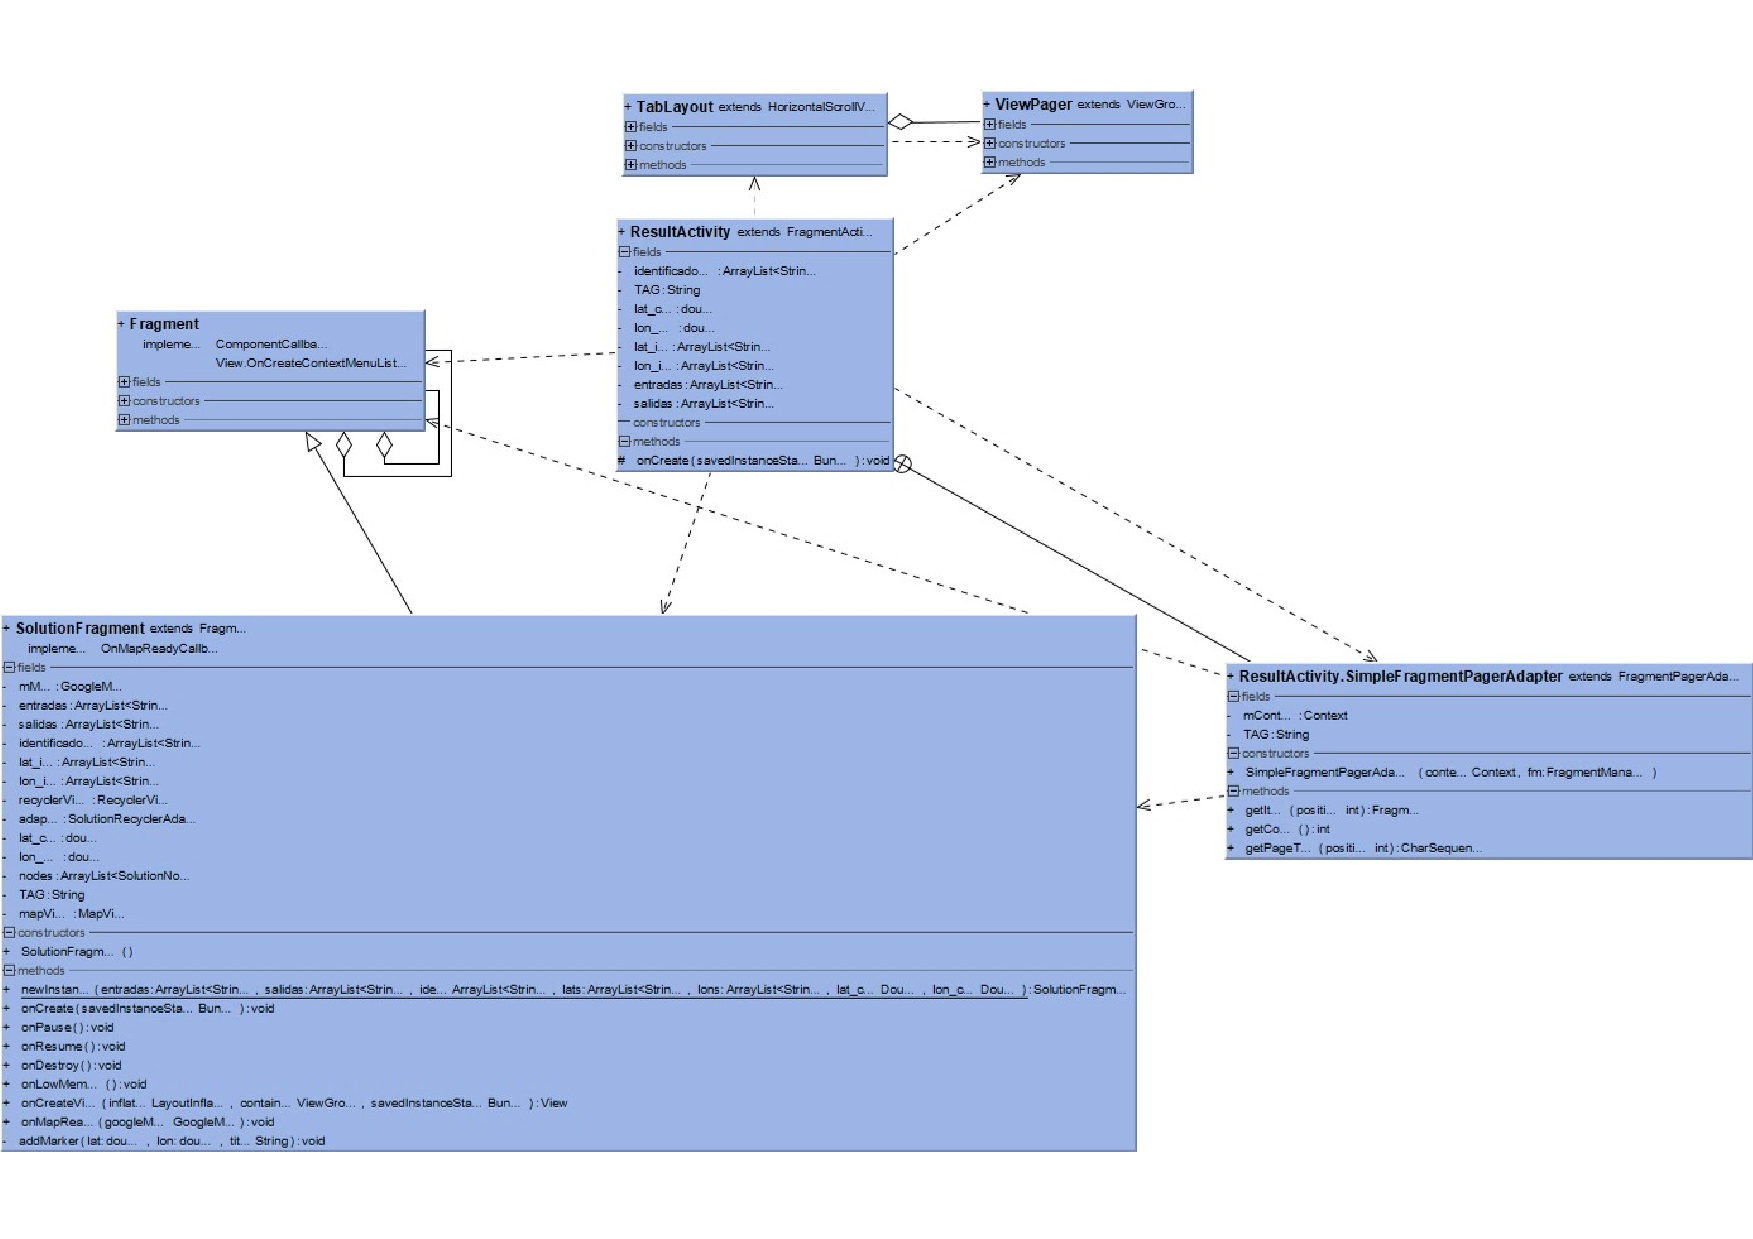
\includegraphics[scale=0.8,angle=90]{imagenes/result_activity.pdf}
	\caption{Diagrama de clases del activity \textbf{ResultActivity}}
	\label{fig:result_activity_diagram}
\end{figure}
\begin{figure}[H]
	\centering
	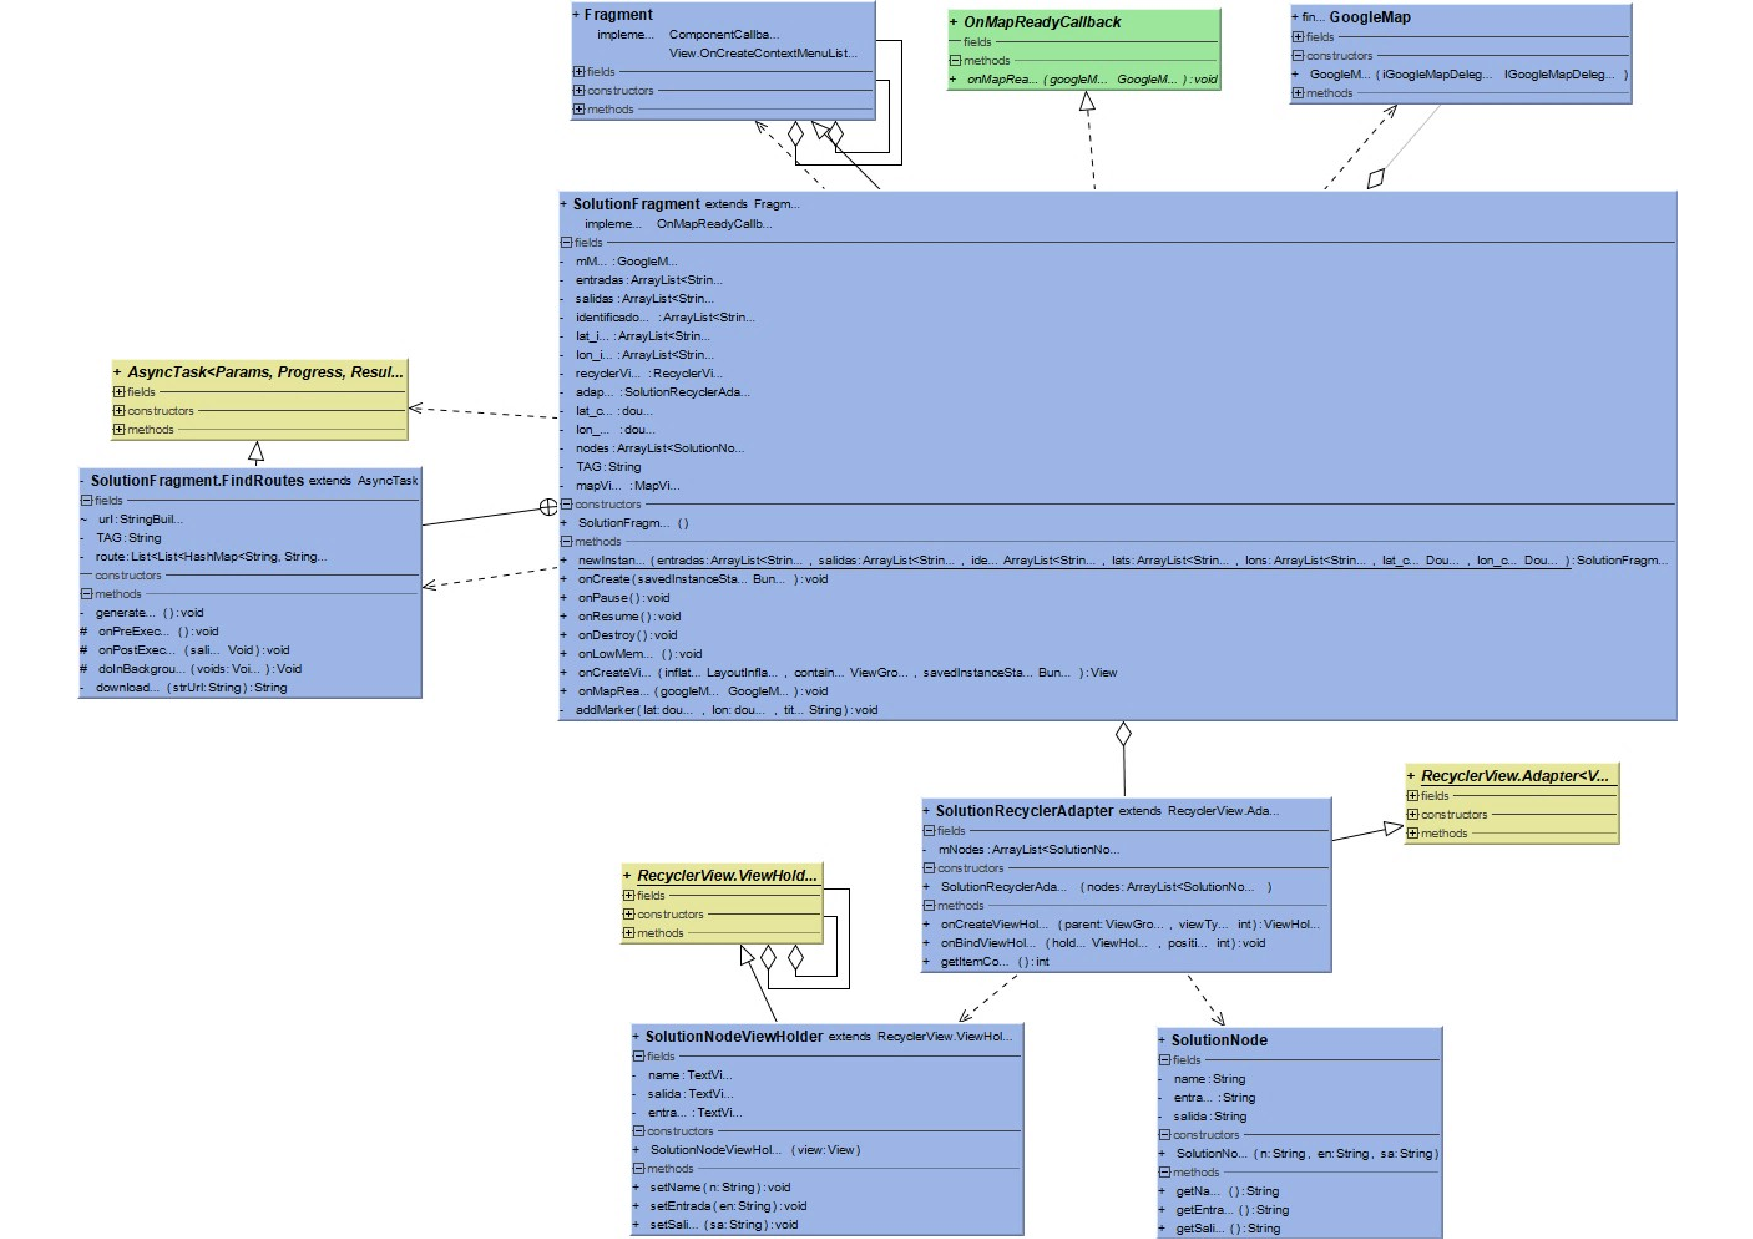
\includegraphics[scale=0.8,angle=90]{imagenes/result_fragment.pdf}
	\caption{Diagrama de clases de la clase \textbf{SolutionFragment}}
	\label{fig:solution_recycler_diagram}
\end{figure}


\section[Interfaz de Usuario]{Interfaz de Usuario}

A continuación se mostrarán todos los elementos que conforman la interfaz de usuario de la aplicación.\newline

Lo primero que se muestra es la actividad principal, esta cuenta con un mapa por el que se puede navegar y una lista de alojamientos y puntos de interés, entre los cuales el usuario puede elegir un alojamiento y el número de puntos de interés que desee; esto se puede encontrar en las figuras \ref{fig:main_activity_map}\ref{fig:main_activity_list}.\newline

Para poder ver la lista, se debe deslizar la pestaña \enquote{Sitios interesantes} hacia arriba, así tendremos acceso a la lista completa, para explorar todos los alojamientos y puntos de interés, debemos hacer scroll hacia arriba sobre la lista. Dicha lista muestra primero los alojamientos y tras estos los puntos de interés, que se organizan en \enquote{Museos}, \enquote{Miradores} y \enquote{Monumentos}.\newline

Dentro la lista, cada uno de los elementos contiene un caja en la que se puede pulsar para seleccionar o deseleccionar de dicho elemento. Dentro de las vistas de los tipos de punto de interés, se encuentra también una caja, dicha caja permite seleccionar o deseleccionar todos los puntos de interés de ese tipo.\newline

Tras elegir el alojamiento los puntos de interés que el usuario desee, se ejecuta el algoritmo y cuando este termina se abre una nueva actividad en la cual se muestran diferentes rutas al problema, por defecto se muestra la primera ruta, para mostrar otras rutas, se debe pulsar sobre los tabs llamados \enquote{"Solución X"} para mostar otras soluciones.\newline

Dentro de cada una de las soluciones, se puede pulsar sobre los marcadores para mostrar información sobre los mismos. Además, en la parte inferior de la pantalla se muestra una lista oculta que muestra la información detalla de la ruta; para poder ver dicha información se debe deslizar hacia arriba en \enquote{Descripción ruta final} o pulsar. Dentro de la lista, se muestra en orden los puntos de interés que contiene la ruta, el primer punto que se muestra es el alojamiento seleccionado; además, cada uno de los puntos de interés muestra la hora aproximada de entrada y de salida de dicho punto de interés. Debajo se muestran figuras de ejemplo sobre esto \ref{fig:result_activity}\ref{fig:result_activity_2}.


\newpage
\begin{figure}[H]
	\centering
	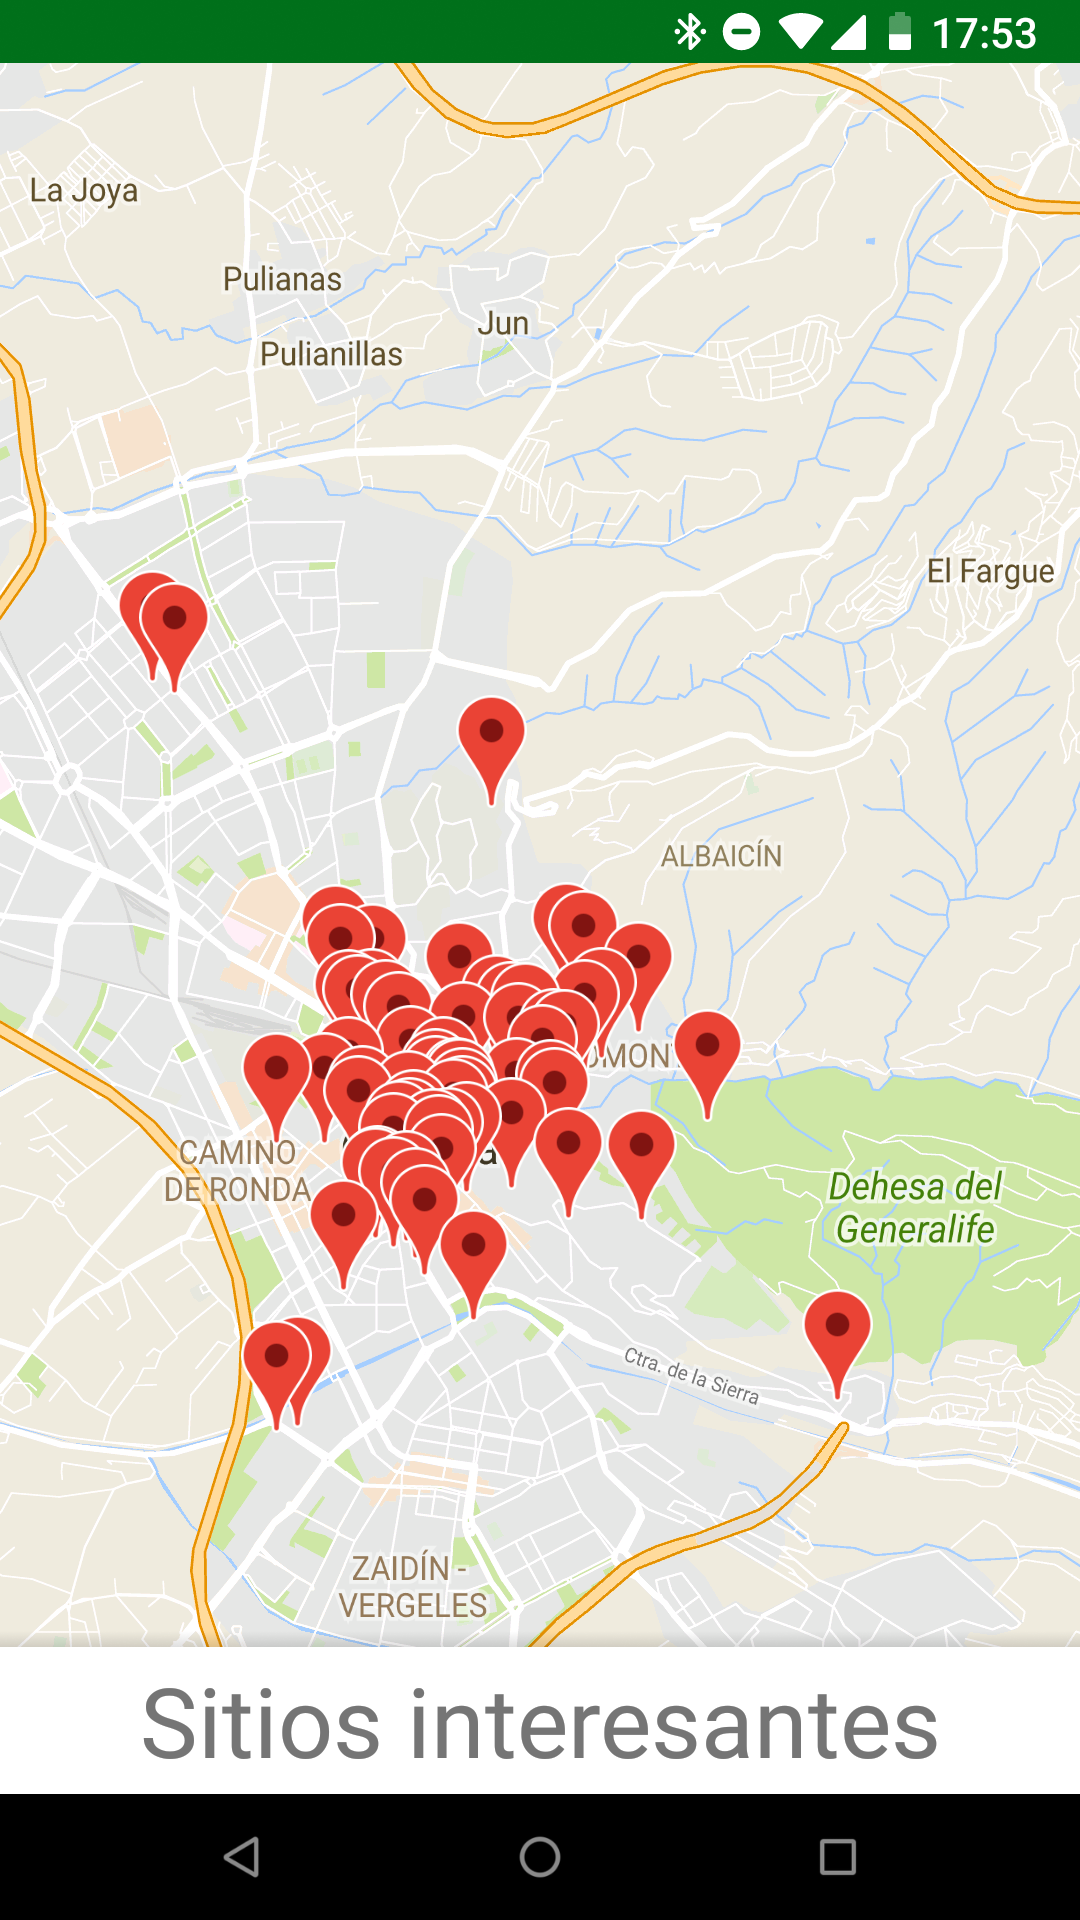
\includegraphics[width=50mm]{imagenes/main_activity_map}
	\caption{Mapa mostrando los puntos de interés y alojamientos sobre el mapa}
	\label{fig:main_activity_map}
\end{figure}
\vspace{0.06in}
\begin{figure}[H]
	\centering
	\subfigure{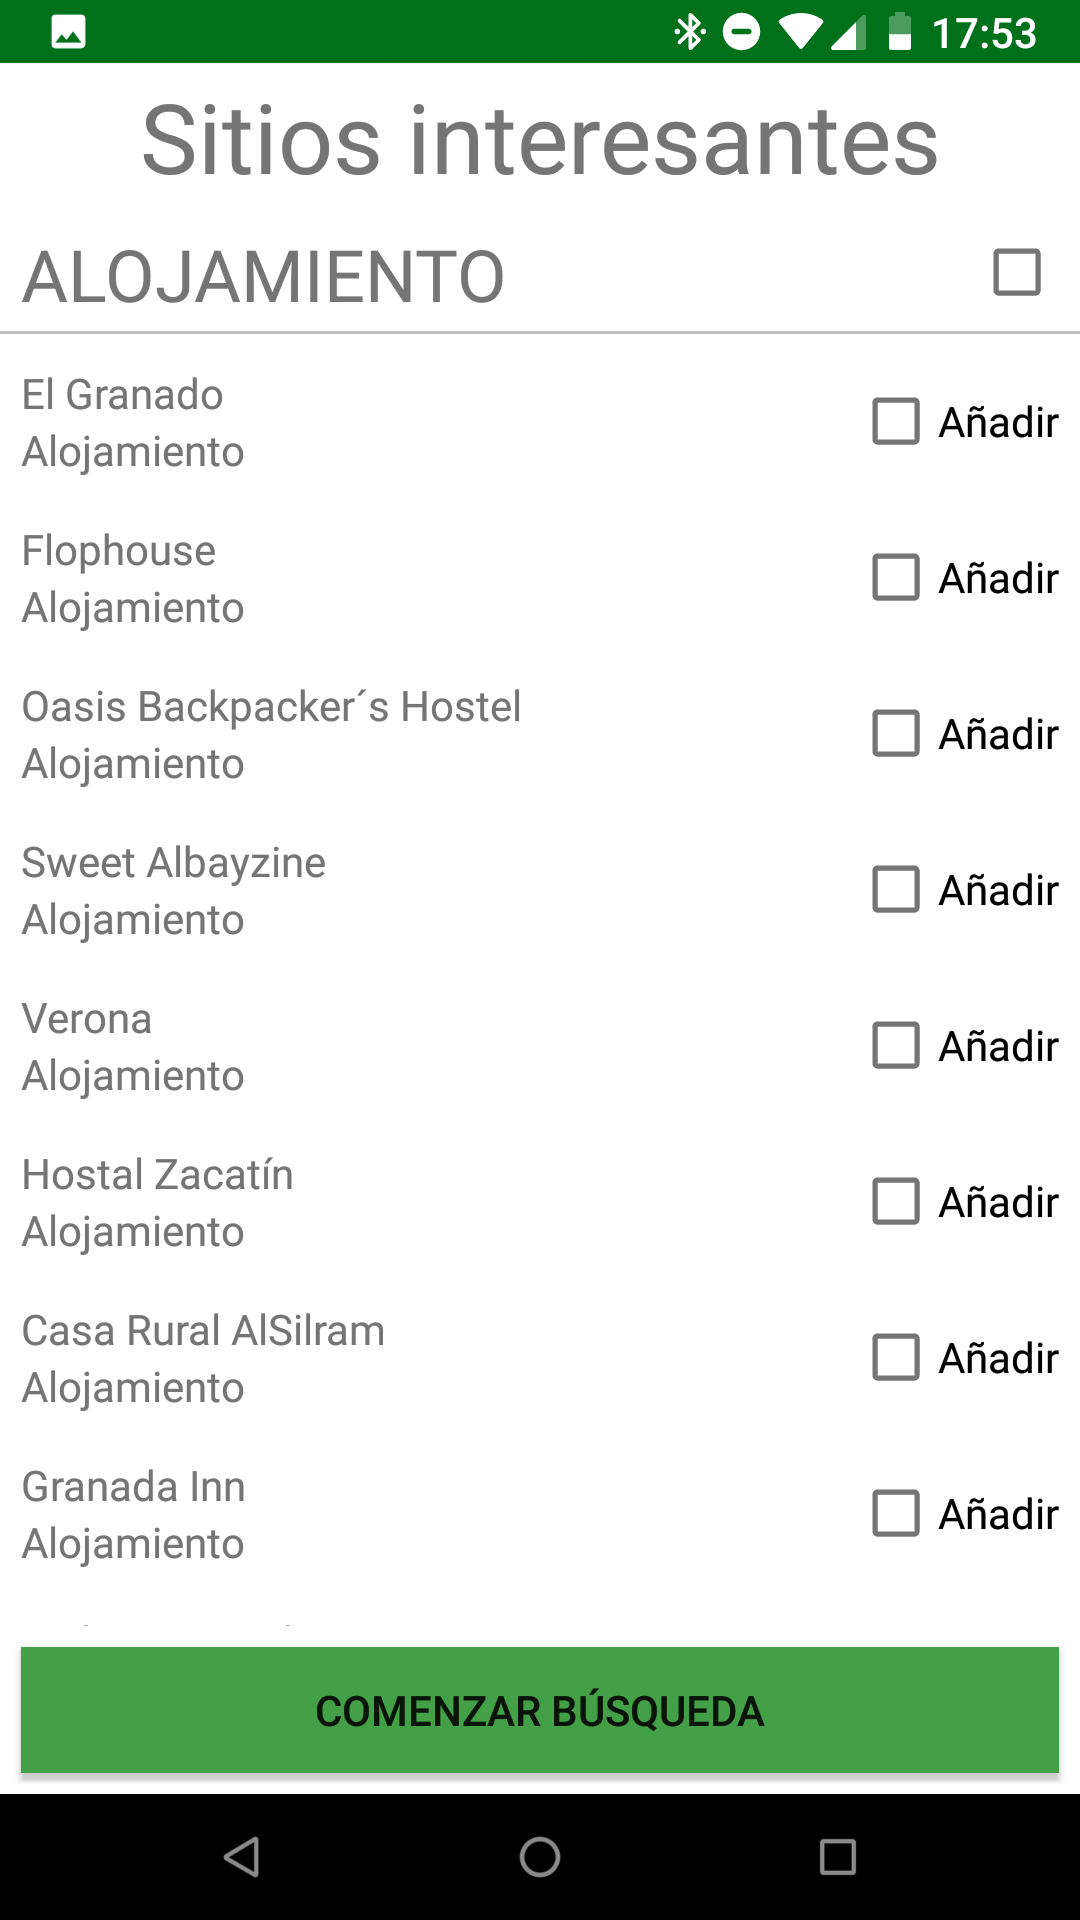
\includegraphics[width=50mm]{imagenes/main_activity_list}}
	\subfigure{
\includegraphics[width=50mm]{imagenes/main_activity_list_2}}
	\caption{Lista de alojamientos y puntos de interés disponibles para seleccionar}
	\label{fig:main_activity_list}
\end{figure}

\vspace{0.06in}
\begin{figure}
	\centering
	\subfigure{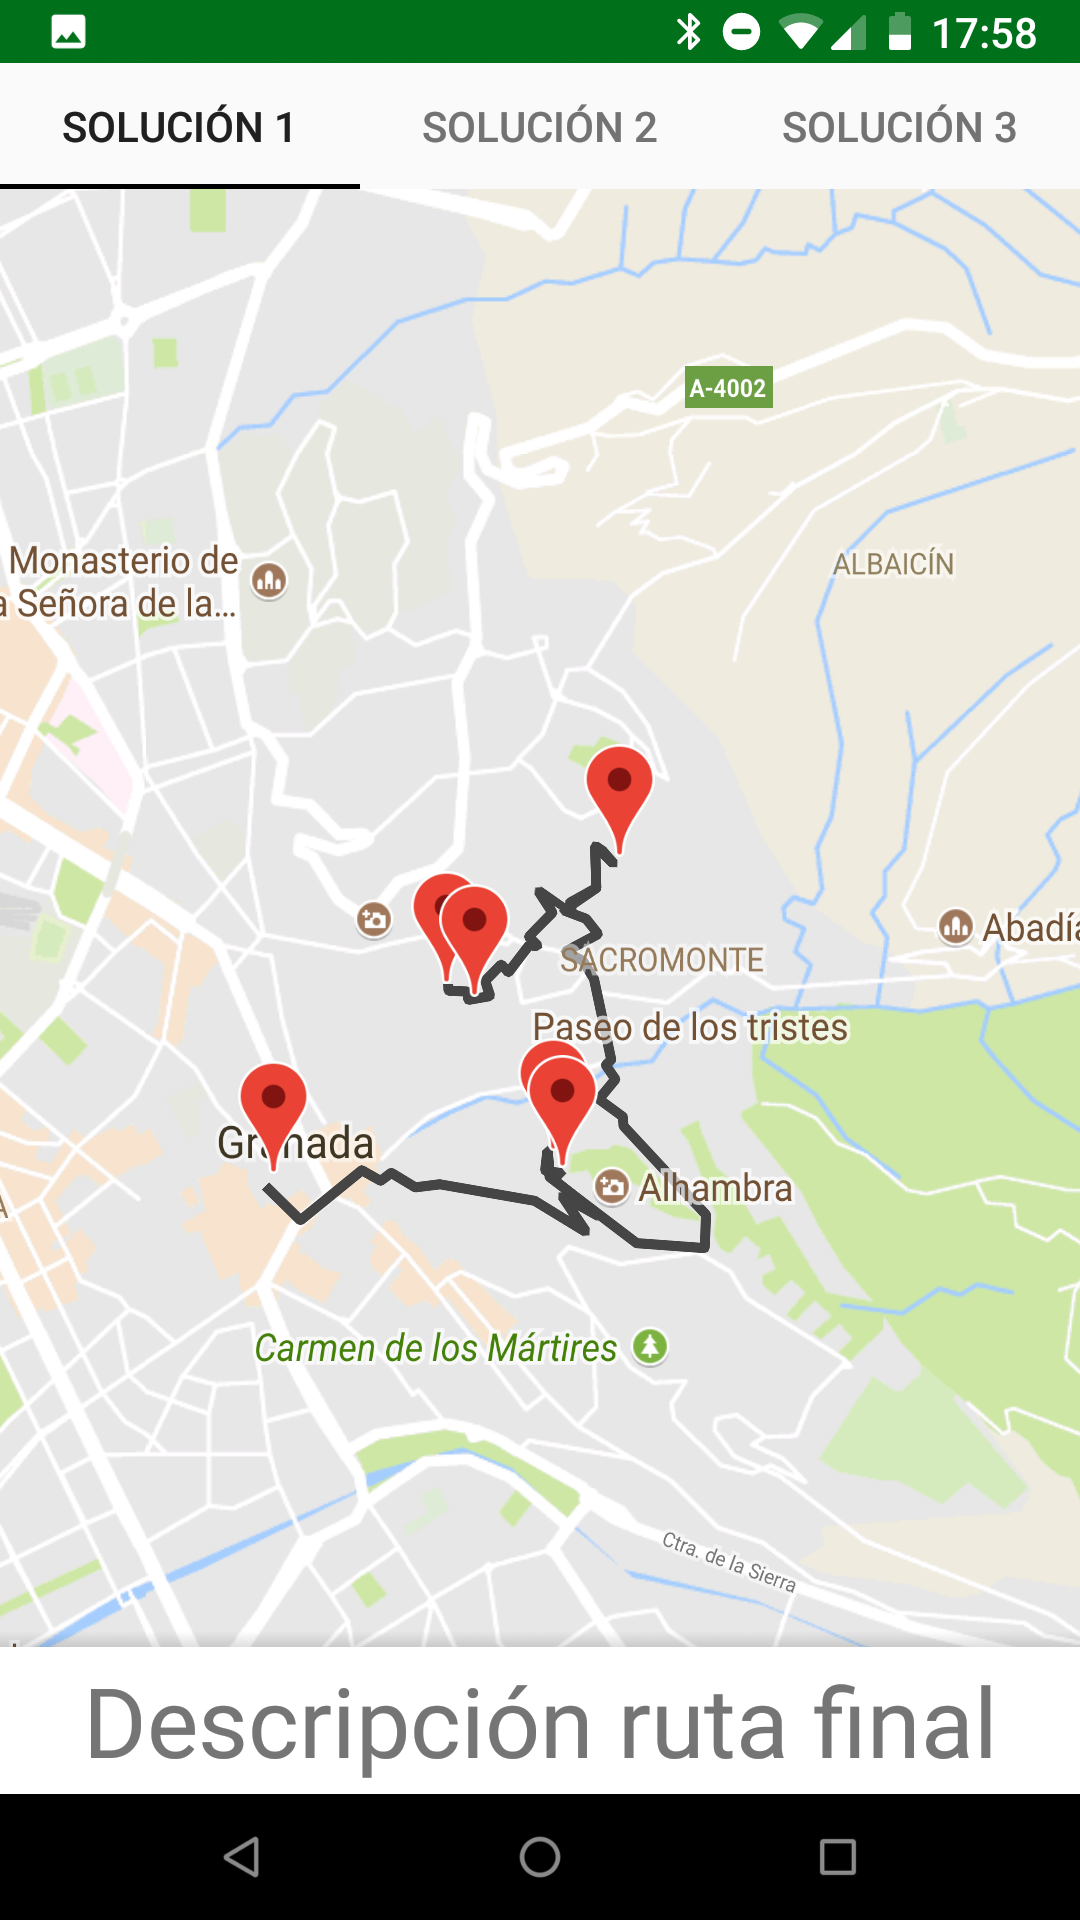
\includegraphics[width=50mm]{imagenes/solution}}
	\subfigure{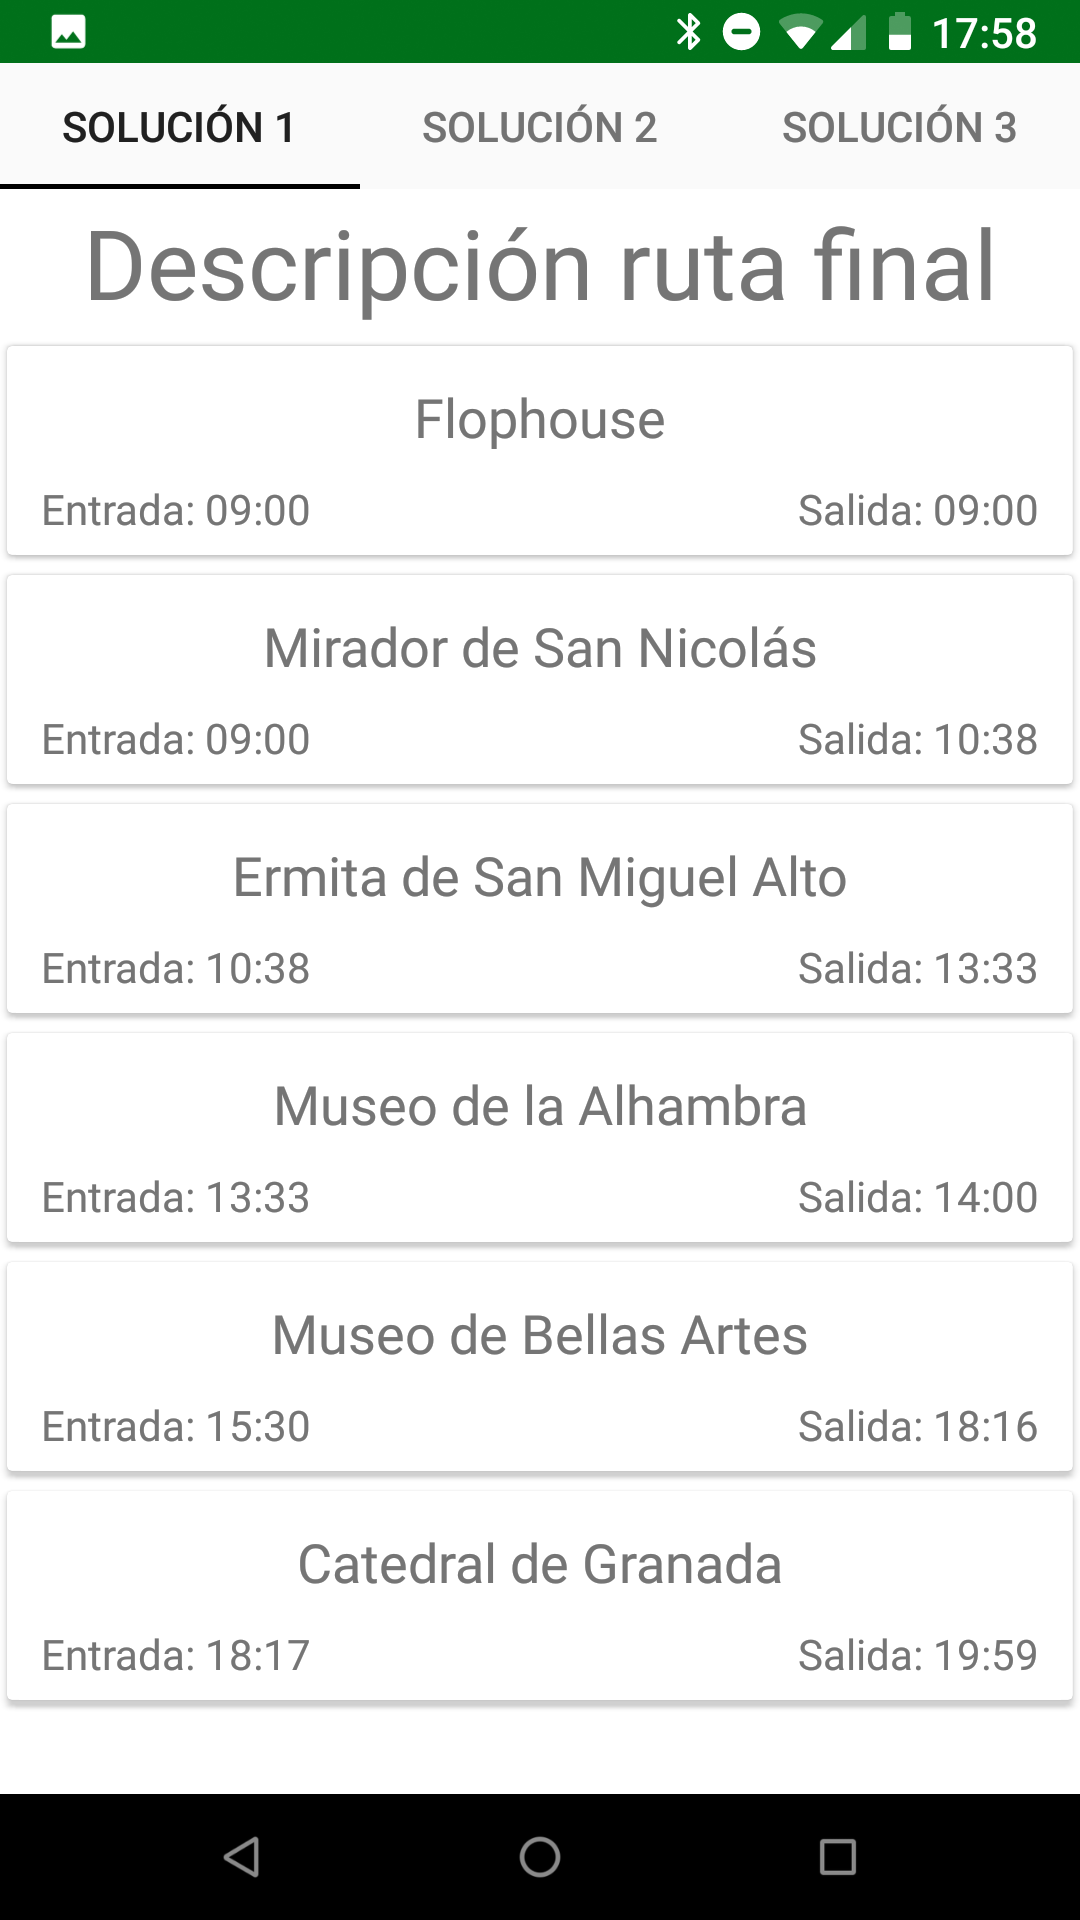
\includegraphics[width=50mm]{imagenes/list_solution}}
	\caption{Mapa mostrando solución y lista de puntos de interés de la solución}
	\label{fig:result_activity}
\end{figure}

\begin{figure}[H]
	\centering
	\subfigure{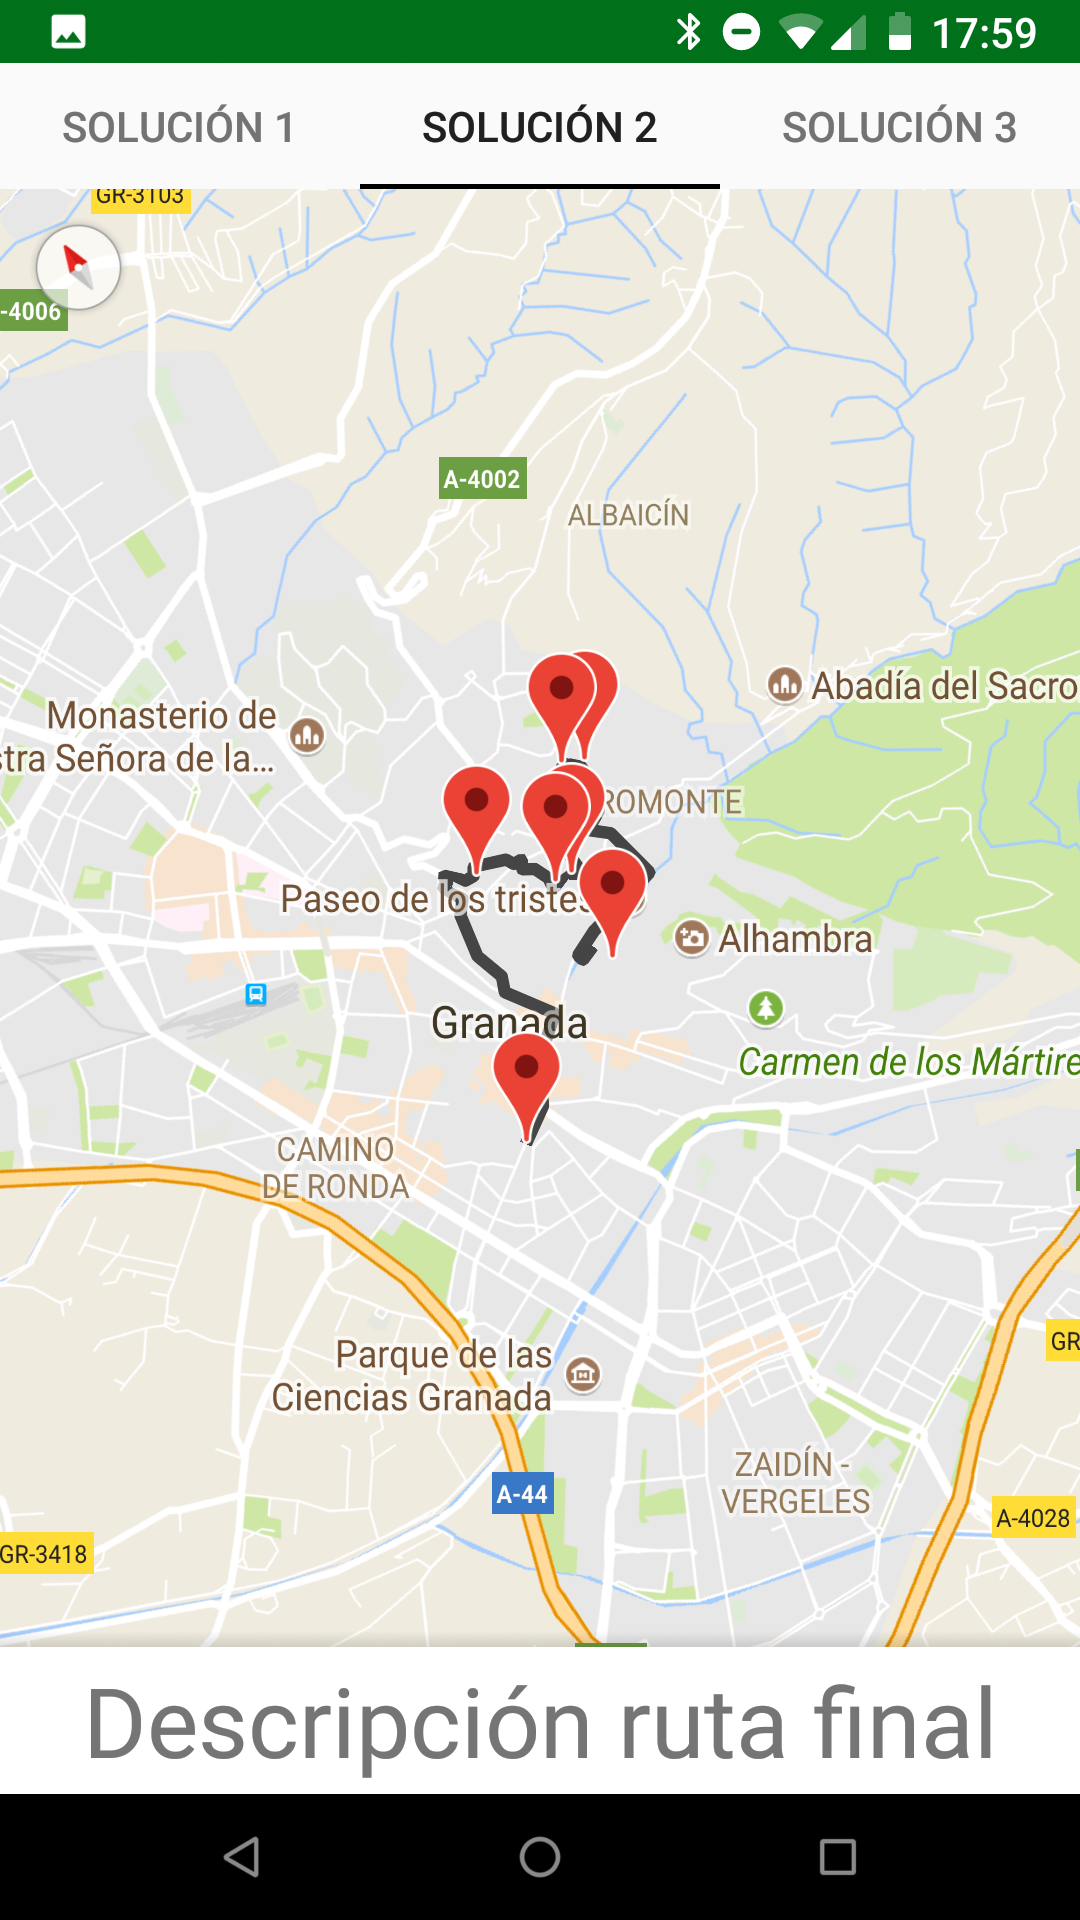
\includegraphics[width=50mm]{imagenes/solution_2}}
	\subfigure{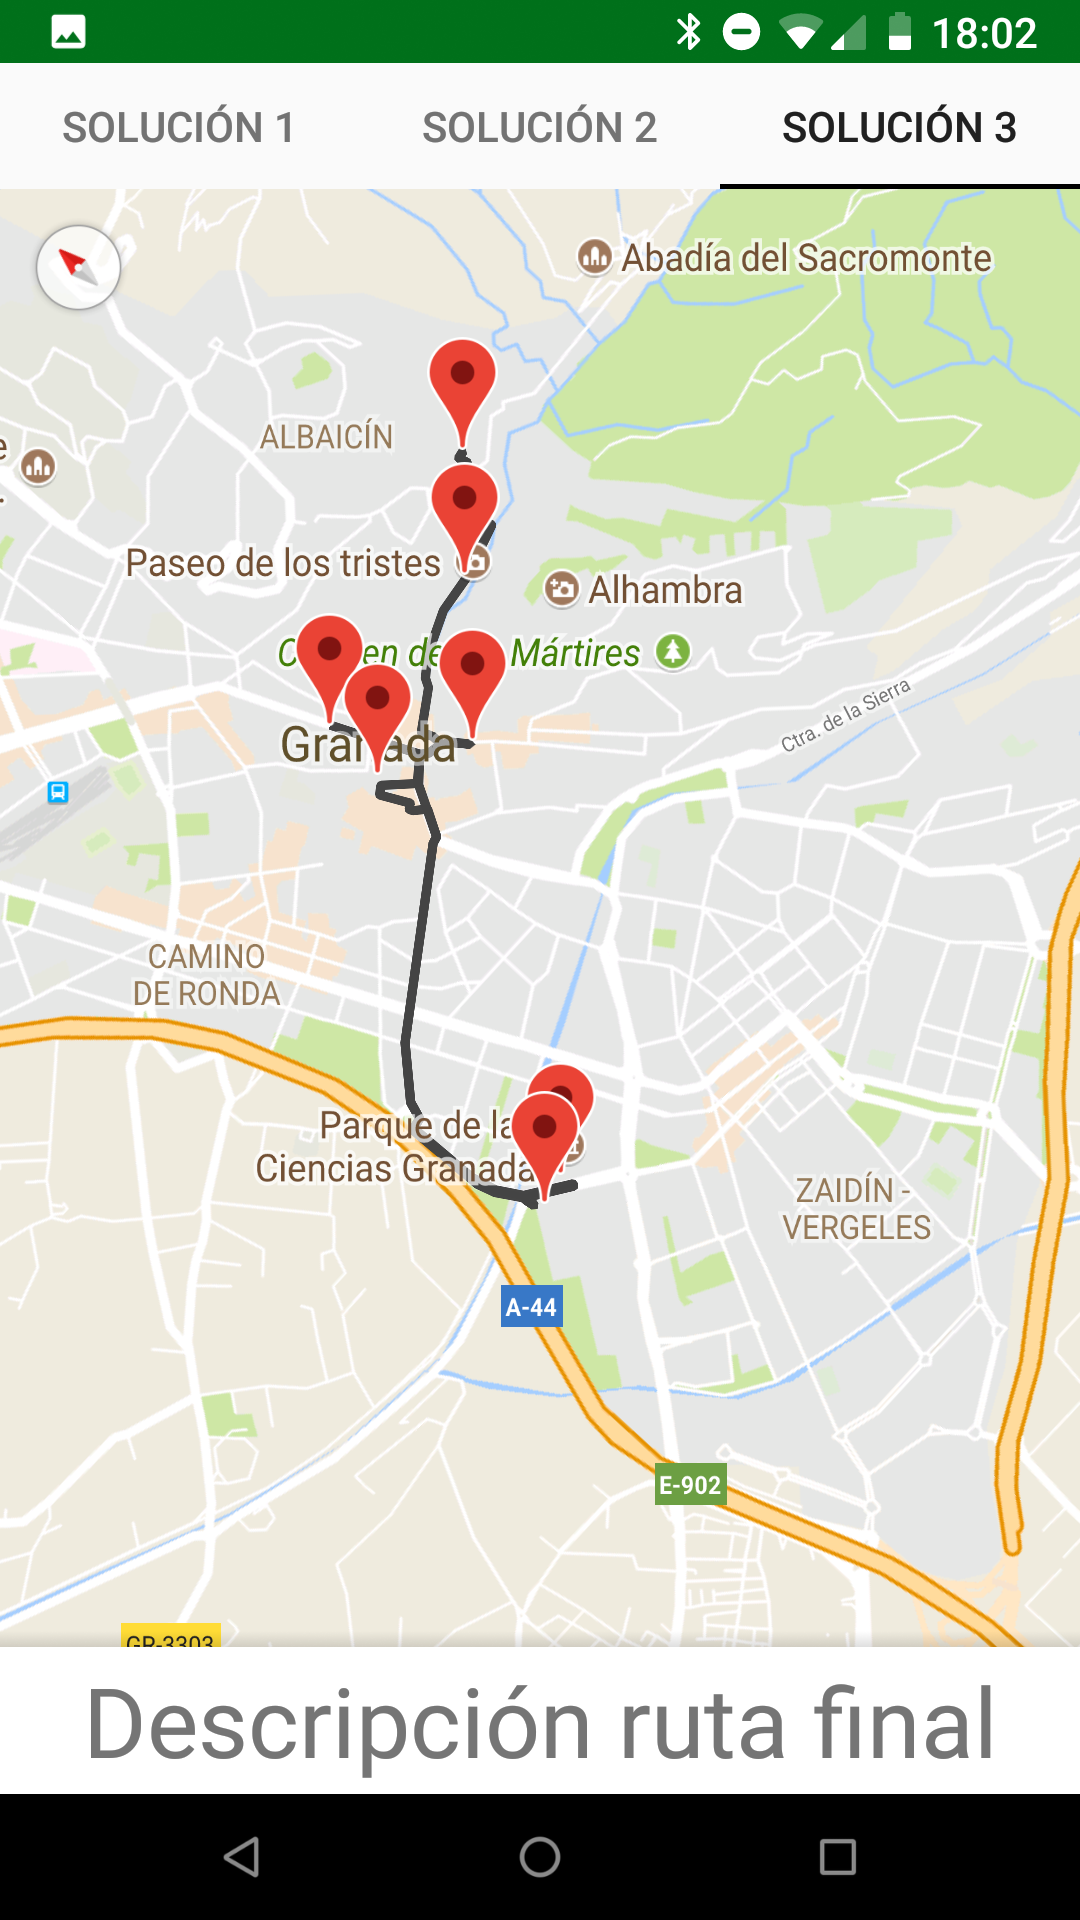
\includegraphics[width=50mm]{imagenes/solution_3}}
	\caption{Diferentes soluciones mostradas en un mapa}
	\label{fig:result_activity_2}
\end{figure}


